\section{Analysis of Potential Confounding Factors} \label{sec:discussion}
In this section, we discuss if the difference of delivery delay between release
strategies could be due to confounding factors, such as the type and the size of
the addressed issues.\\
\begin{figure}
	\centering
	\subfloat[Files]{
		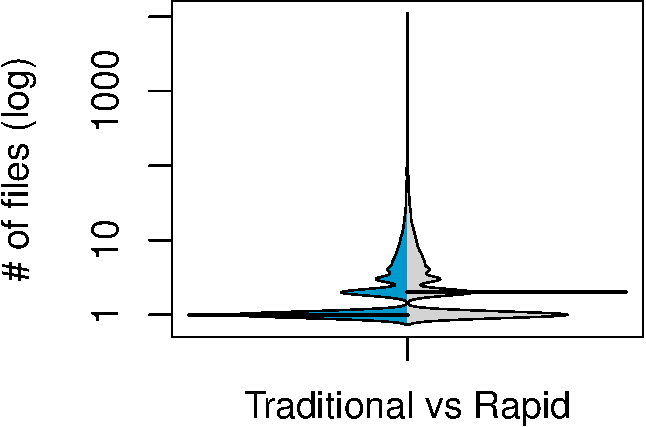
\includegraphics[width=0.3\textwidth,keepaspectratio]
		{chapters/chapter5/figures/rapid-vs-traditional-files.pdf}
	}
	\subfloat[LOC]{
		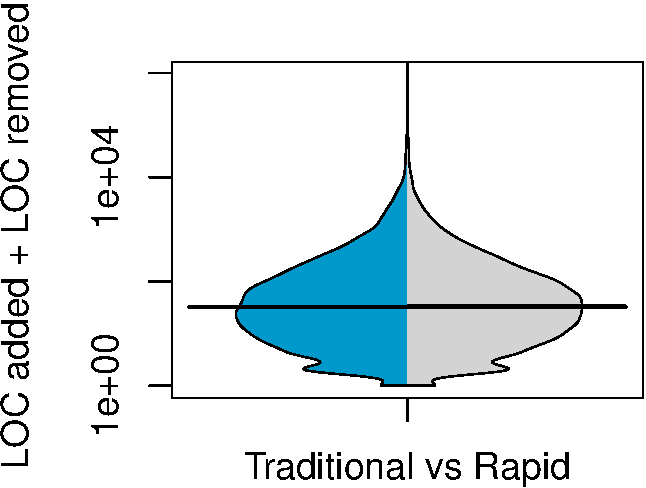
\includegraphics[width=0.3\textwidth,keepaspectratio]
		{chapters/chapter5/figures/discussion/rapid-vs-traditional-churn.pdf}
	}
	\subfloat[Packages]{
		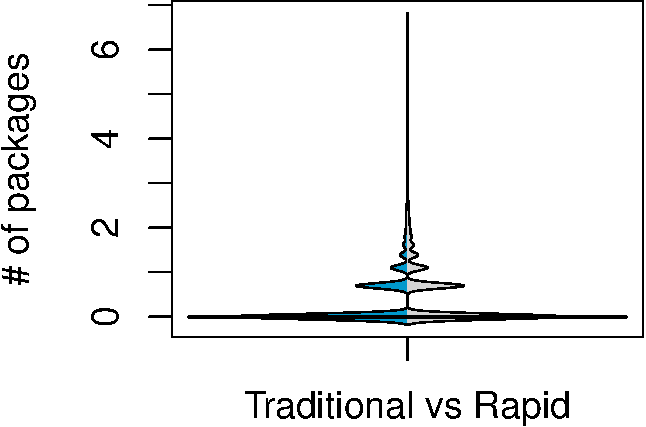
\includegraphics[width=0.3\textwidth,keepaspectratio]
		{chapters/chapter5/figures/discussion/rapid-vs-traditional-packages.pdf}
	}
	\caption{Size of the addressed issues in the traditional and rapid release data.}
	\label{fig:issue_granularity}
\end{figure}

\noindent\textit{\textbf{Observation~8---The delivery delay of addressed issues is unlikely to be
related to the size of an issue.}}\observation{obs:8}
One may suspect that the difference in delivery delay between release
strategies may be due to the \textit{size of an issue}. We use the
\textit{number of files}, \textit{LOC}, and \textit{number of packages} that
were involved in the fix of an issue to measure the \textit{size of an issue}.
\hyperref[fig:issue_granularity]{Figure}~\ref{fig:issue_granularity} shows the
distributions of the metrics that measure the \textit{size of an issue}.  We
observe that the difference between distributions of \textit{LOC} is
statistically insignificant~($p=0.86$). As for the \textit{number of files} and
the \textit{number of packages}, although we observe significant differences
($p$ values of $0.014$ and $<2.2e^{-16}$, respectively), effect-sizes are
$negligible$ ($delta=-0.05$ and $delta=-0.07$, respectively).\\

\begin{figure}[!]
	\centering
	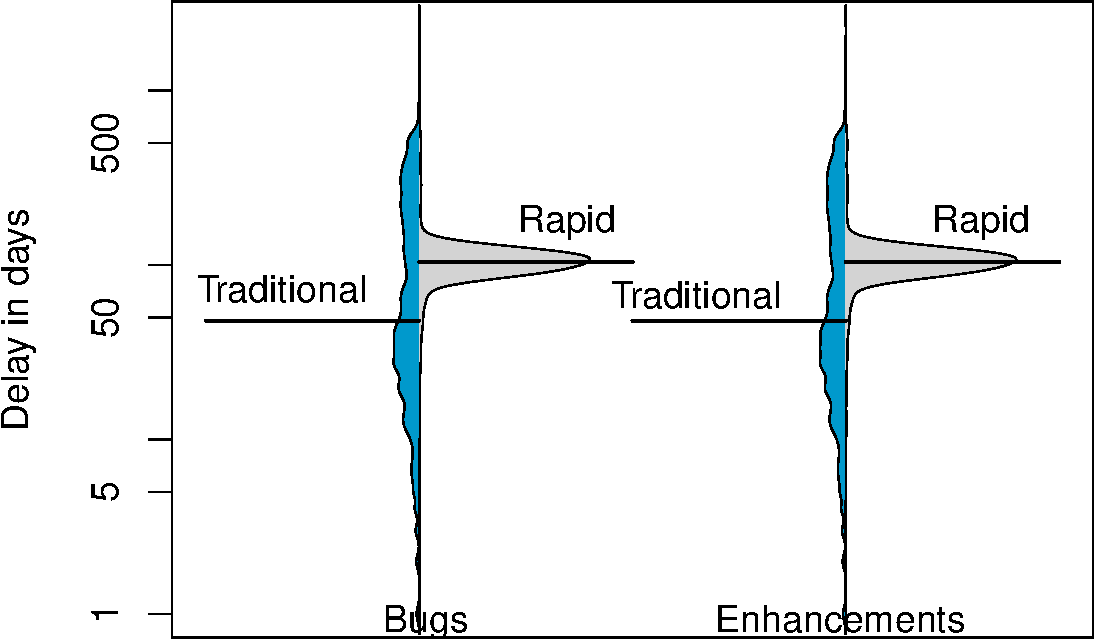
\includegraphics[width=\columnwidth,keepaspectratio]
	{chapters/chapter5/figures/discussion/bugs_vs_enhancements.pdf}
	\caption{We group the addressed issues into ``bugs'' and
	``enhancements'' by using the \textit{severity} field.  However, the
difference in the delivery delay between release strategies is unlikely to be
related with the type of the issue.}
	\label{fig:bugs_vs_enhancements}
\end{figure}

\noindent\textit{\textbf{Observation~9---The difference between traditional and rapid releases
is unlikely to be related to the differences between enhancements and bug
fixes.}}\observation{obs:9}
We also investigate if the observed difference in the delivery delay between
traditional and rapid releases is related to the type of addressed issues. For
example, rapid releases could be delivering more enhancements, which likely
require additional integration time in order to ensure that the new content is
of sufficient quality.
\hyperref[fig:bugs_vs_enhancements]{Figure}~\ref{fig:bugs_vs_enhancements} shows
the distributions of delays among release strategies grouped by bug fixes and
enhancements. We observe no clear distinction between delivery delay and the
type of addressed issues that is being delivered.

